\chapter{Rank Distributions}
\label{appendix:distributions}

\begin{figure}
    \centering
    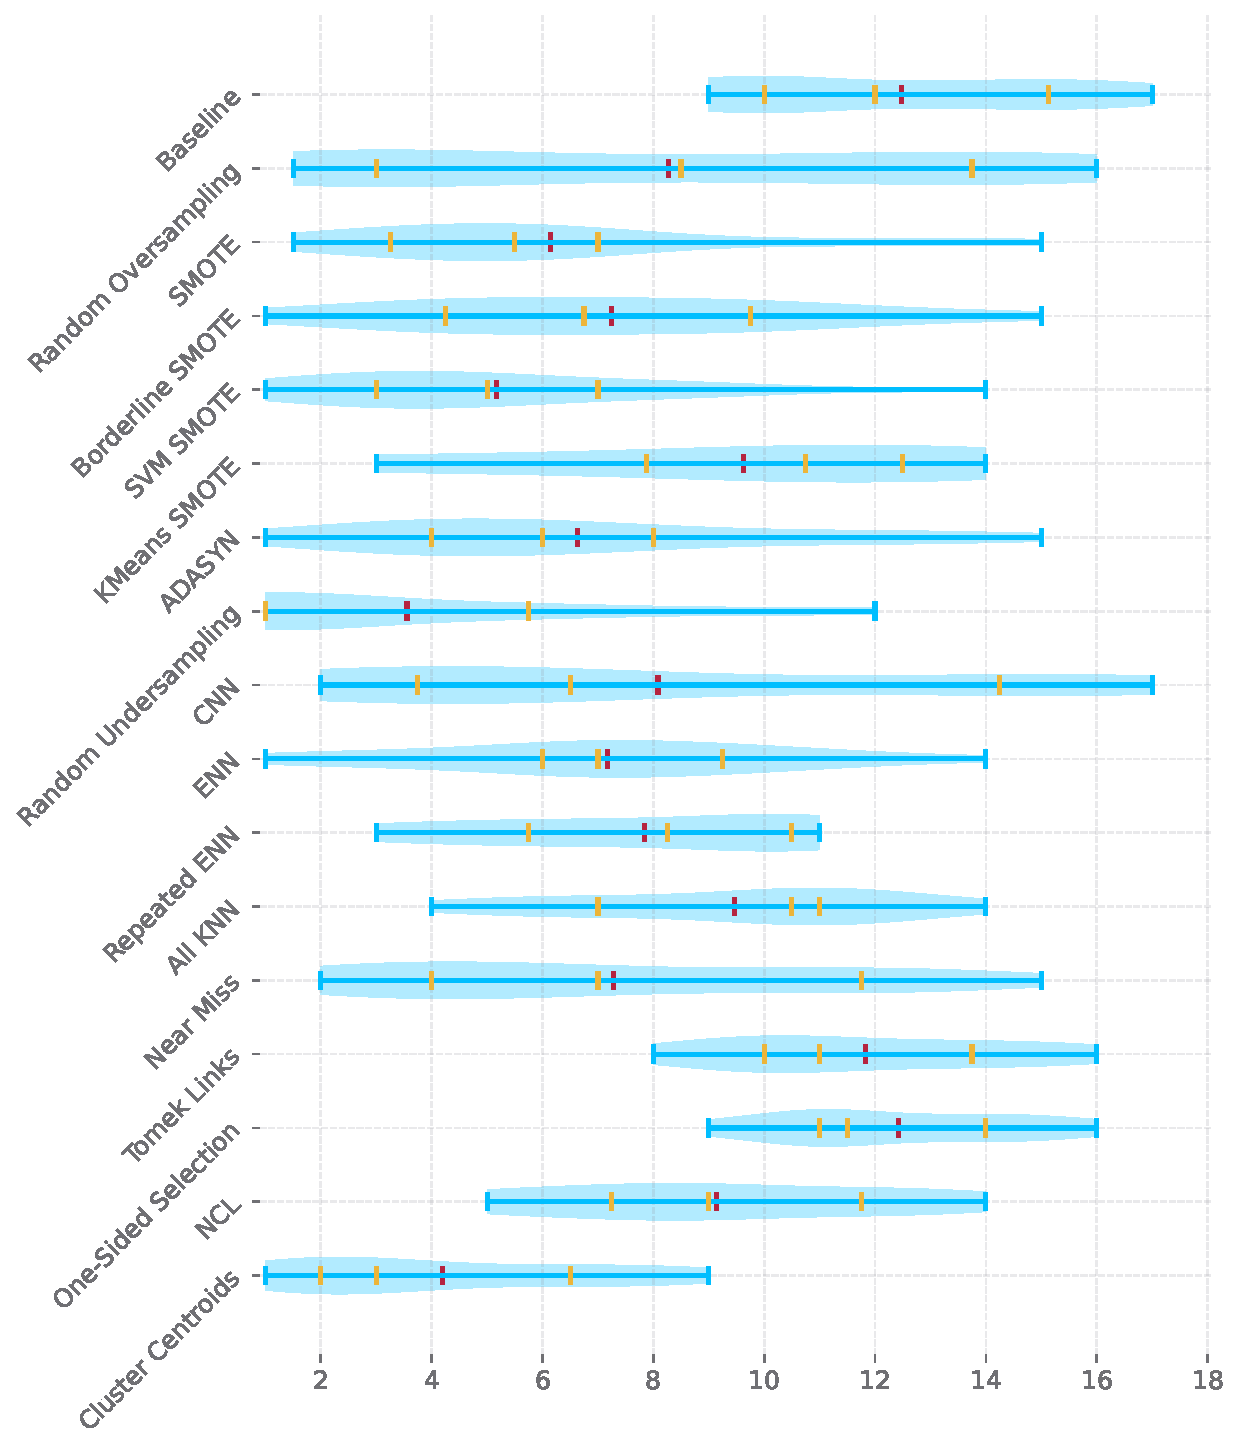
\includegraphics[width=\linewidth]{figures/balanced_accuracy_ranks_distribution.pdf}
    \caption{
        \textbf{Distribution of Ranks for Balanced Accuracy Evaluation Metric.} The figure shows the
        distribution of ranks computed across all datasets in the experiments. Ranks were computed
        from Balanced Accuracy scores for each preprocessing method separately. The red mark
        denotes each method’s mean rank, and three yellow marks indicate the 25th, 50th and 75th
        percentile.
    }
    \label{figure:balanced_accuracy_rank_distributions}
\end{figure}

\begin{figure}
    \centering
    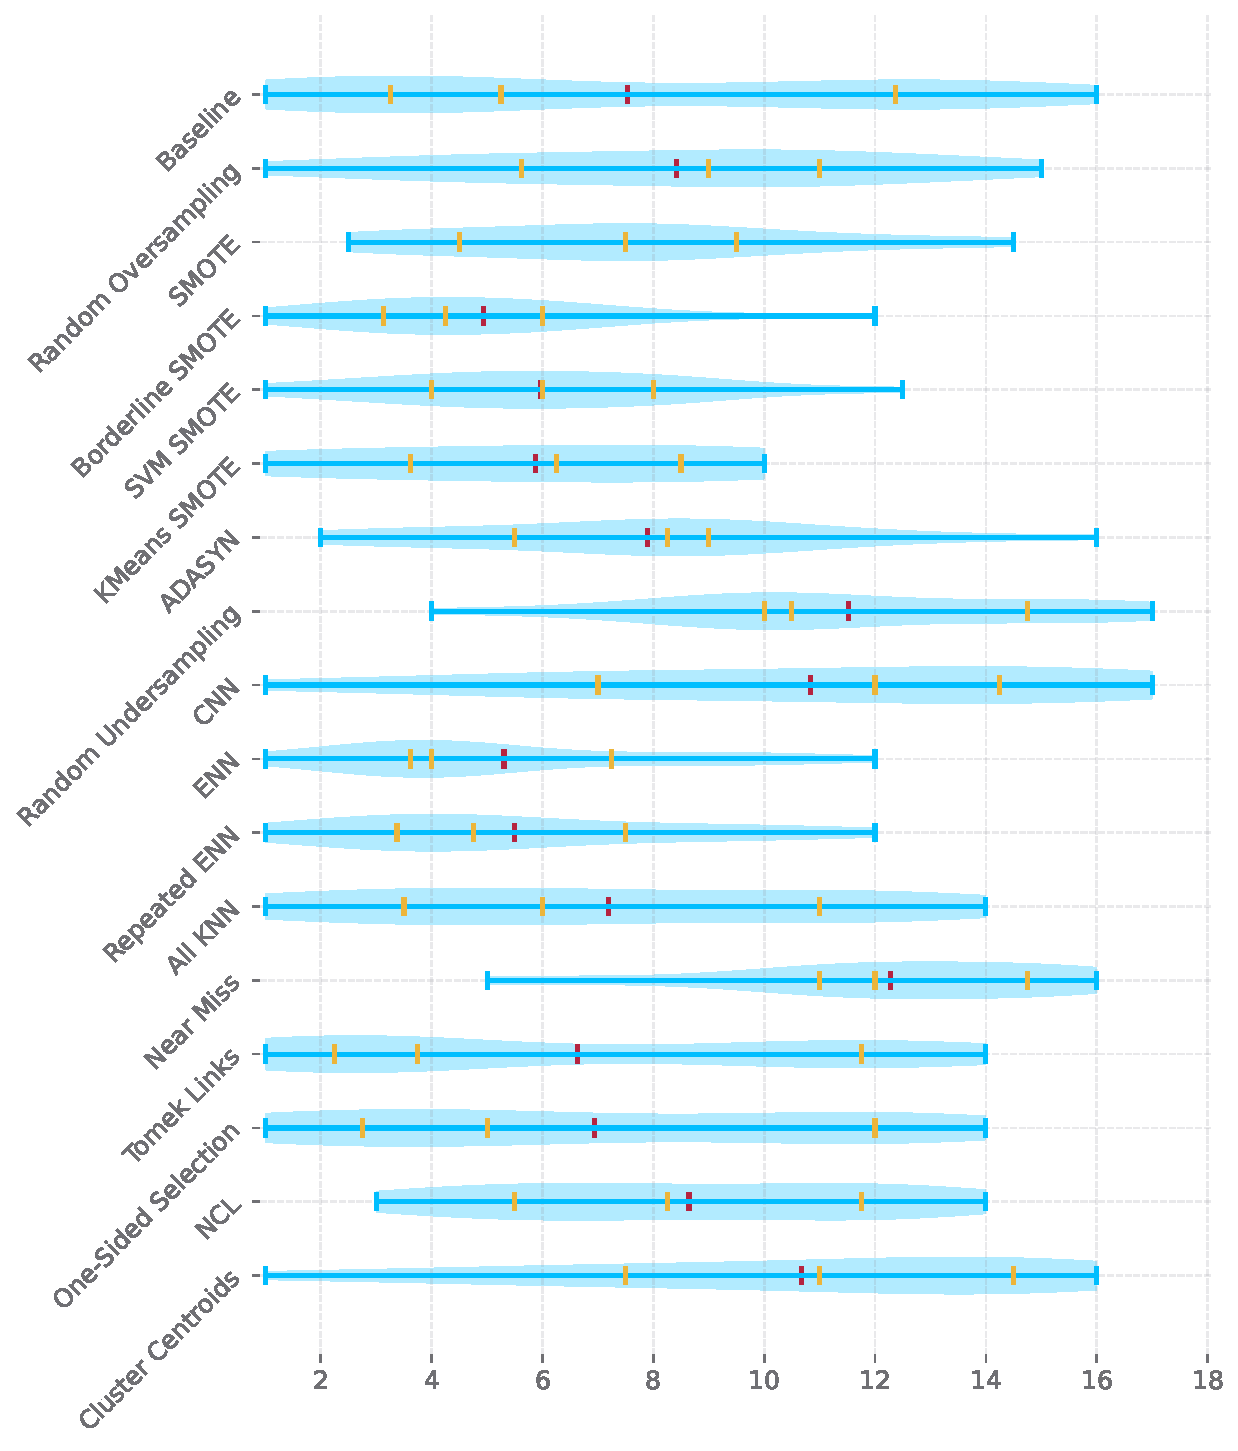
\includegraphics[width=\linewidth]{figures/precision_ranks_distribution.pdf}
    \caption{
        \textbf{Distribution of Ranks for Precision Evaluation Metric.} The figure shows the
        distribution of ranks computed across all datasets in the experiments. Ranks were computed
        from Precision scores for each preprocessing method separately. The red mark denotes each
        method’s mean rank, and three yellow marks indicate the 25th, 50th and 75th percentile.
    }
    \label{figure:precision_rank_distributions}
\end{figure}

\begin{figure}
    \centering
    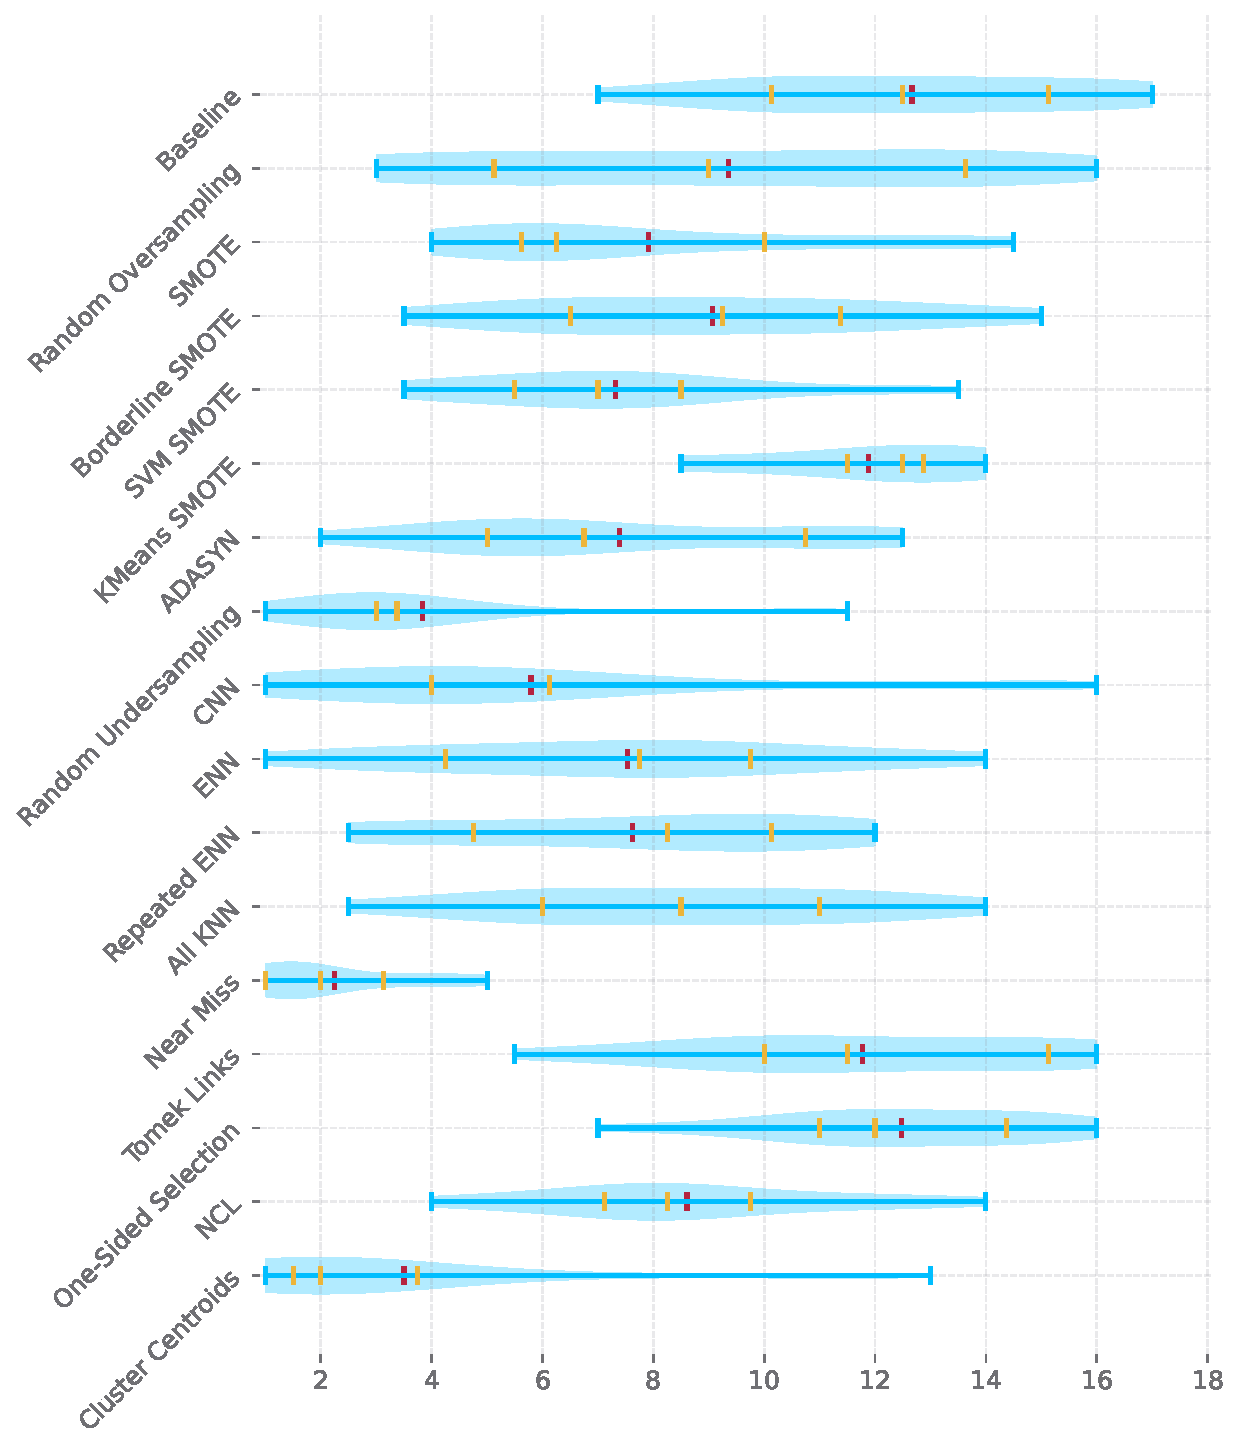
\includegraphics[width=\linewidth]{figures/recall_ranks_distribution.pdf}
    \caption{
        \textbf{Distribution of Ranks for Recall Evaluation Metric.} The figure shows the
        distribution of ranks computed across all datasets in the experiments. Ranks were computed
        from Recall scores for each preprocessing method separately. The red mark denotes each
        method’s mean rank, and three yellow marks indicate the 25th, 50th and 75th percentile.
    }
    \label{figure:recall_rank_distributions}
\end{figure}

\begin{figure}
    \centering
    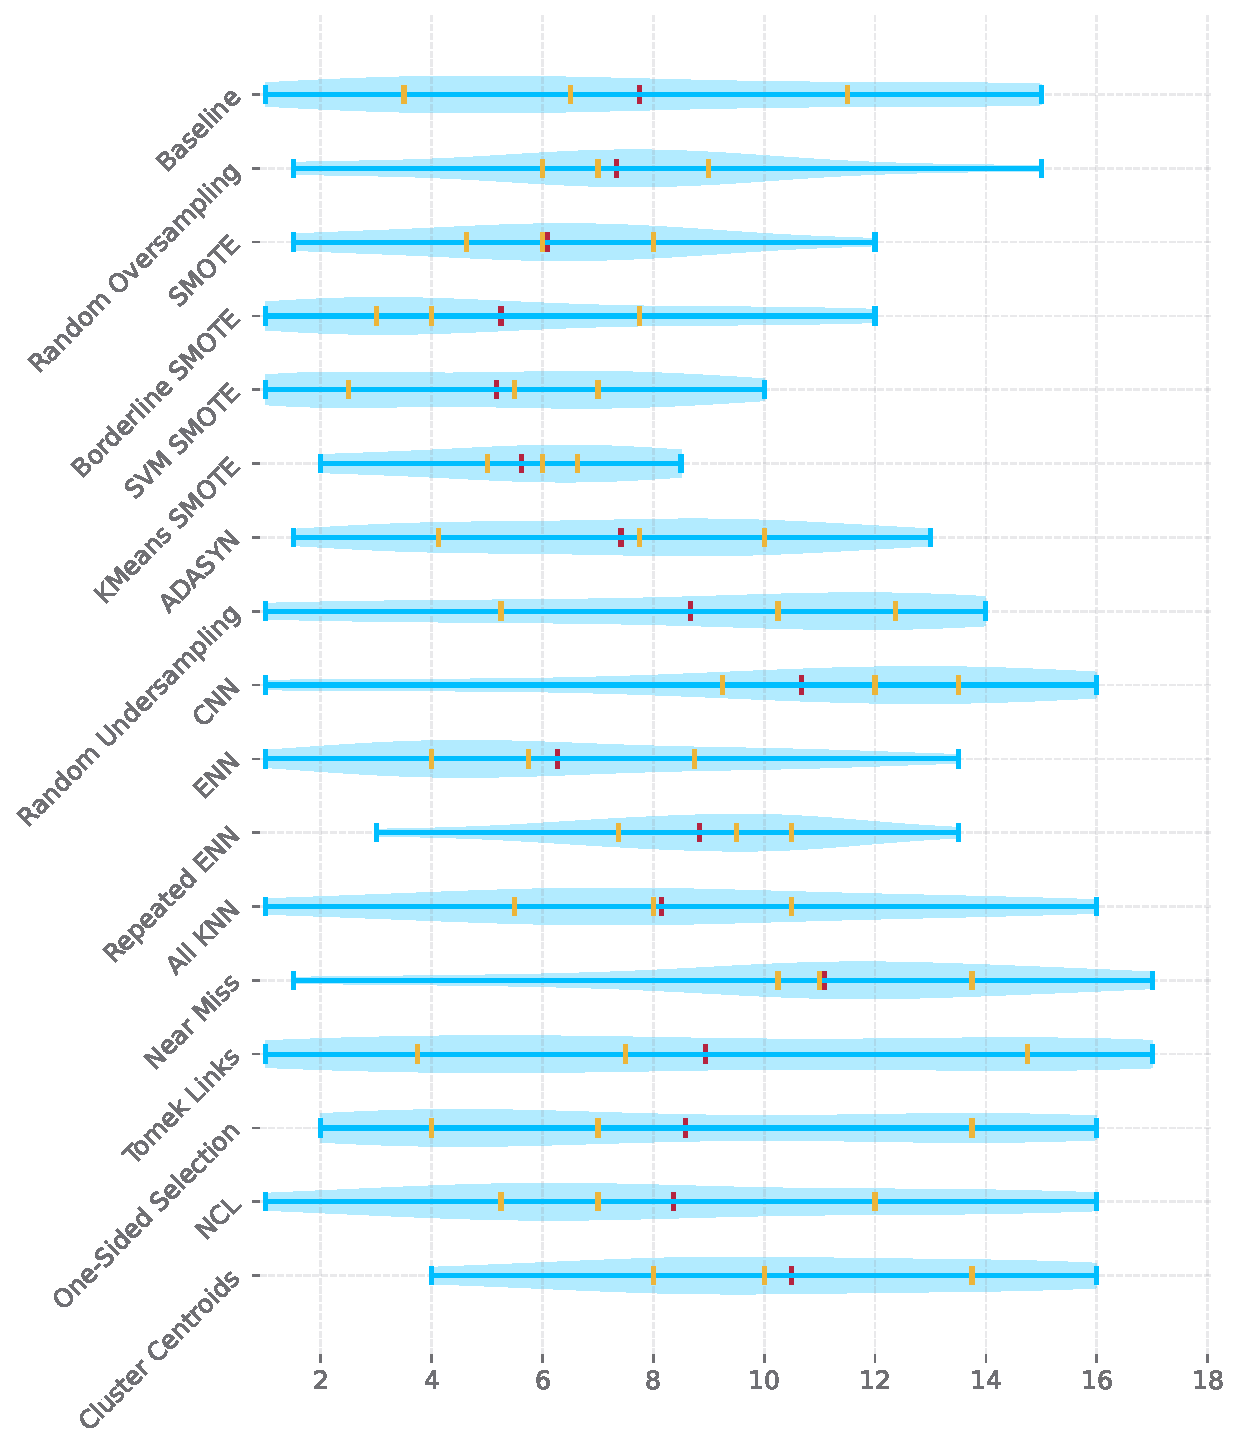
\includegraphics[width=\linewidth]{figures/f1_max_ranks_distribution.pdf}
    \caption{
        \textbf{Distribution of Ranks for F1 Max Evaluation Metric.} The figure shows the
        distribution of ranks computed across all datasets in the experiments. Ranks were computed
        from F1 Max scores for each preprocessing method separately. The red mark denotes each
        method’s mean rank, and three yellow marks indicate the 25th, 50th and 75th percentile.
    }
    \label{figure:f1_max_rank_distributions}
\end{figure}

\begin{figure}
    \centering
    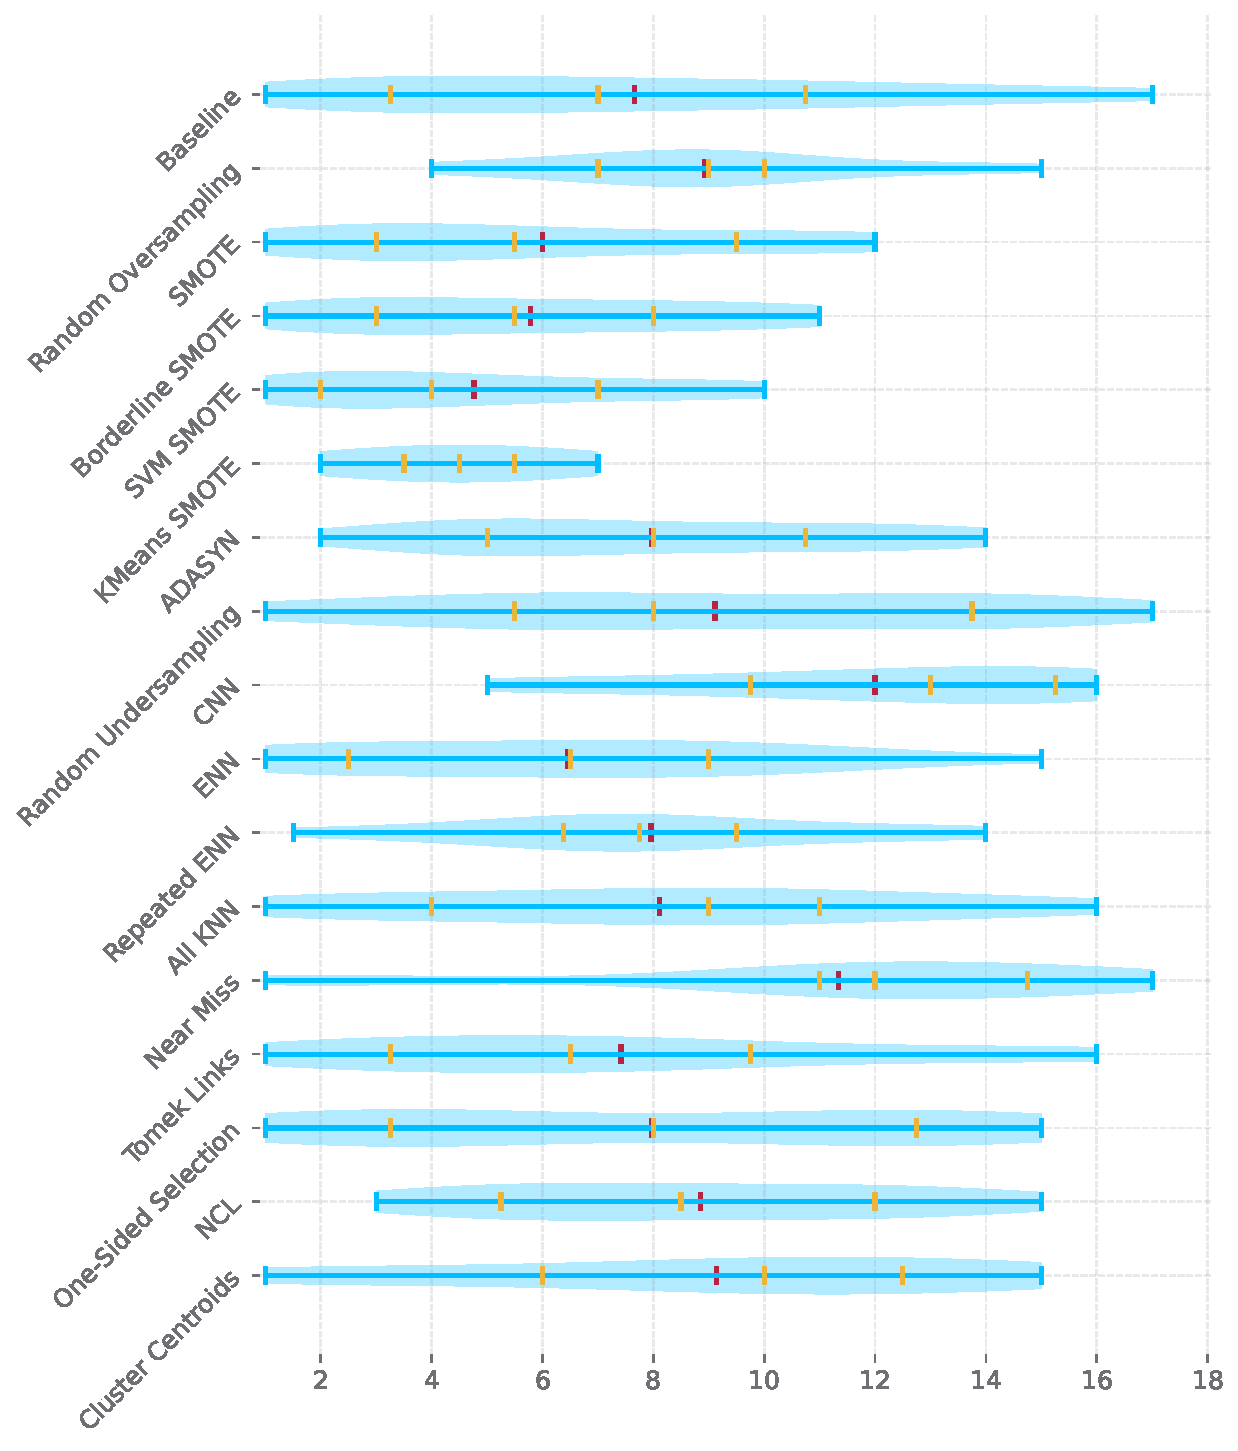
\includegraphics[width=\linewidth]{figures/pr_auc_ranks_distribution.pdf}
    \caption{
        \textbf{Distribution of Ranks for PR AUC Evaluation Metric.} The figure shows the
        distribution of ranks computed across all datasets in the experiments. Ranks were computed
        from PR AUC scores for each preprocessing method separately. The red mark denotes each
        method’s mean rank, and three yellow marks indicate the 25th, 50th and 75th percentile.
    }
    \label{figure:pr_auc_rank_distributions}
\end{figure}

\begin{figure}
    \centering
    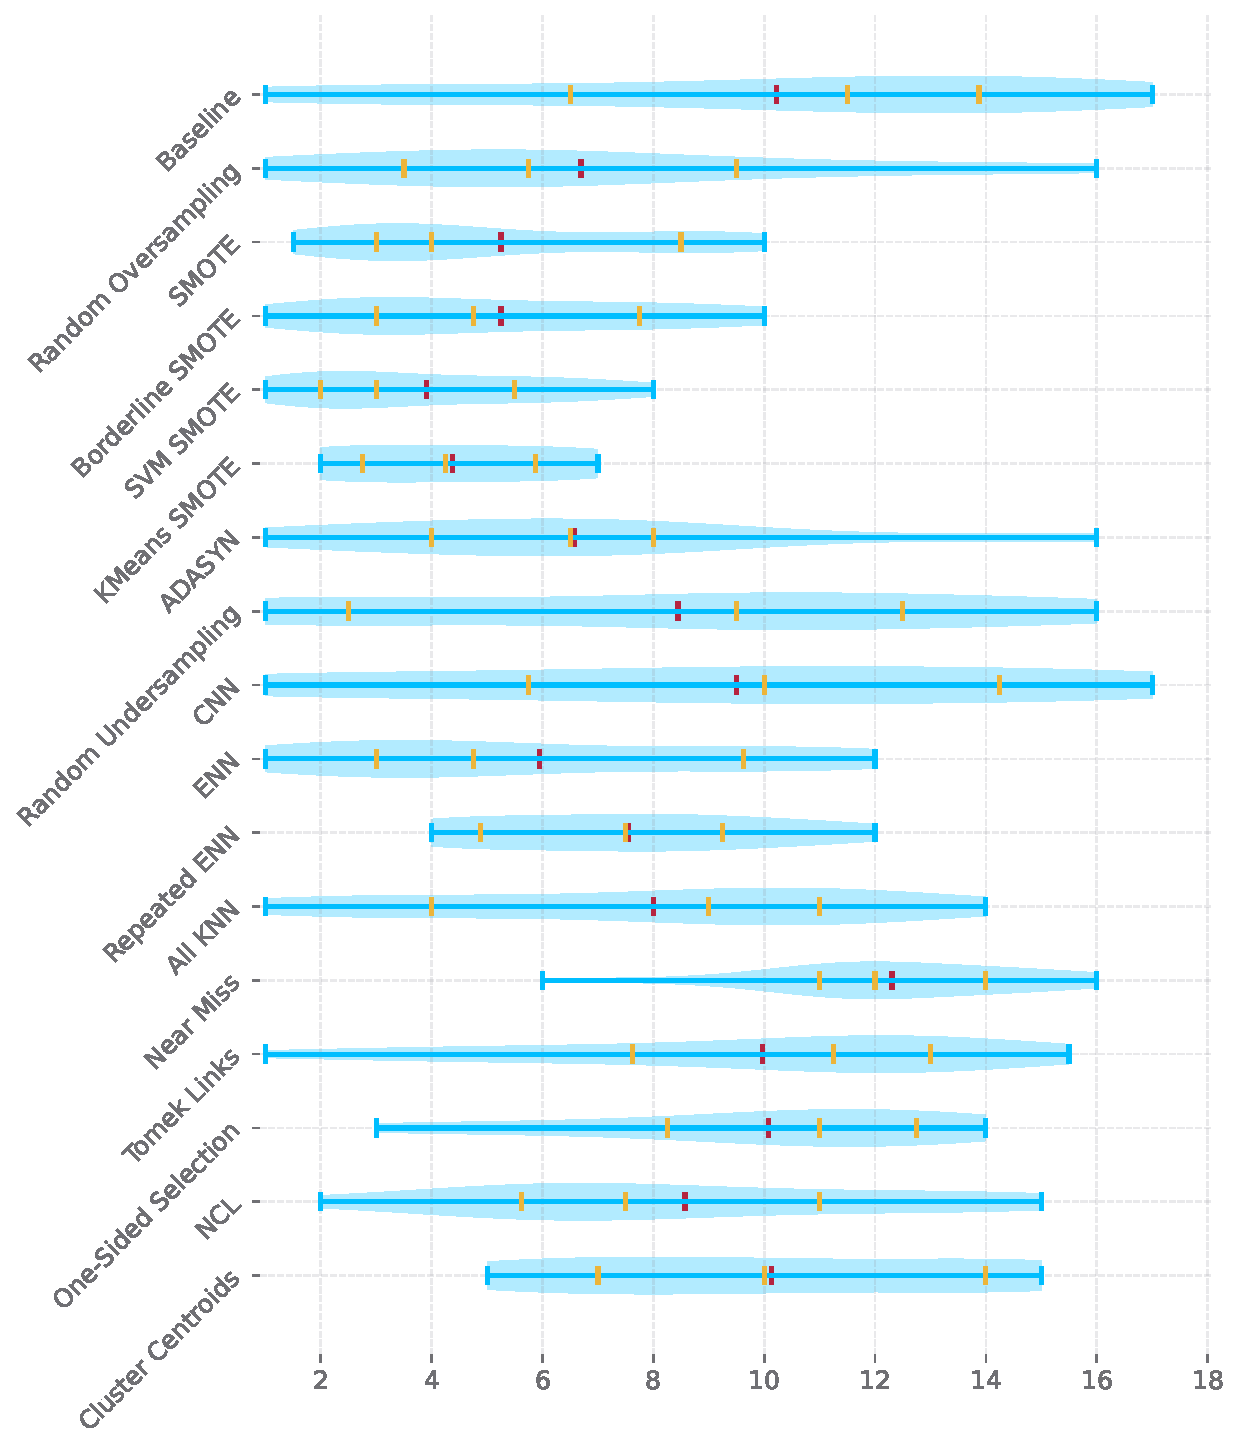
\includegraphics[width=\linewidth]{figures/matthews_corr_coef_ranks_distribution.pdf}
    \caption{
        \textbf{Distribution of Ranks for Matthews Correlation Coefficient Evaluation Metric.} The
        figure shows the distribution of ranks computed across all datasets in the experiments.
        Ranks were computed from MCC scores for each preprocessing method separately. The red mark
        denotes each method’s mean rank, and three yellow marks indicate the 25th, 50th and 75th
        percentile.
    }
    \label{figure:mcc_rank_distributions}
\end{figure}

\begin{figure}
    \centering
    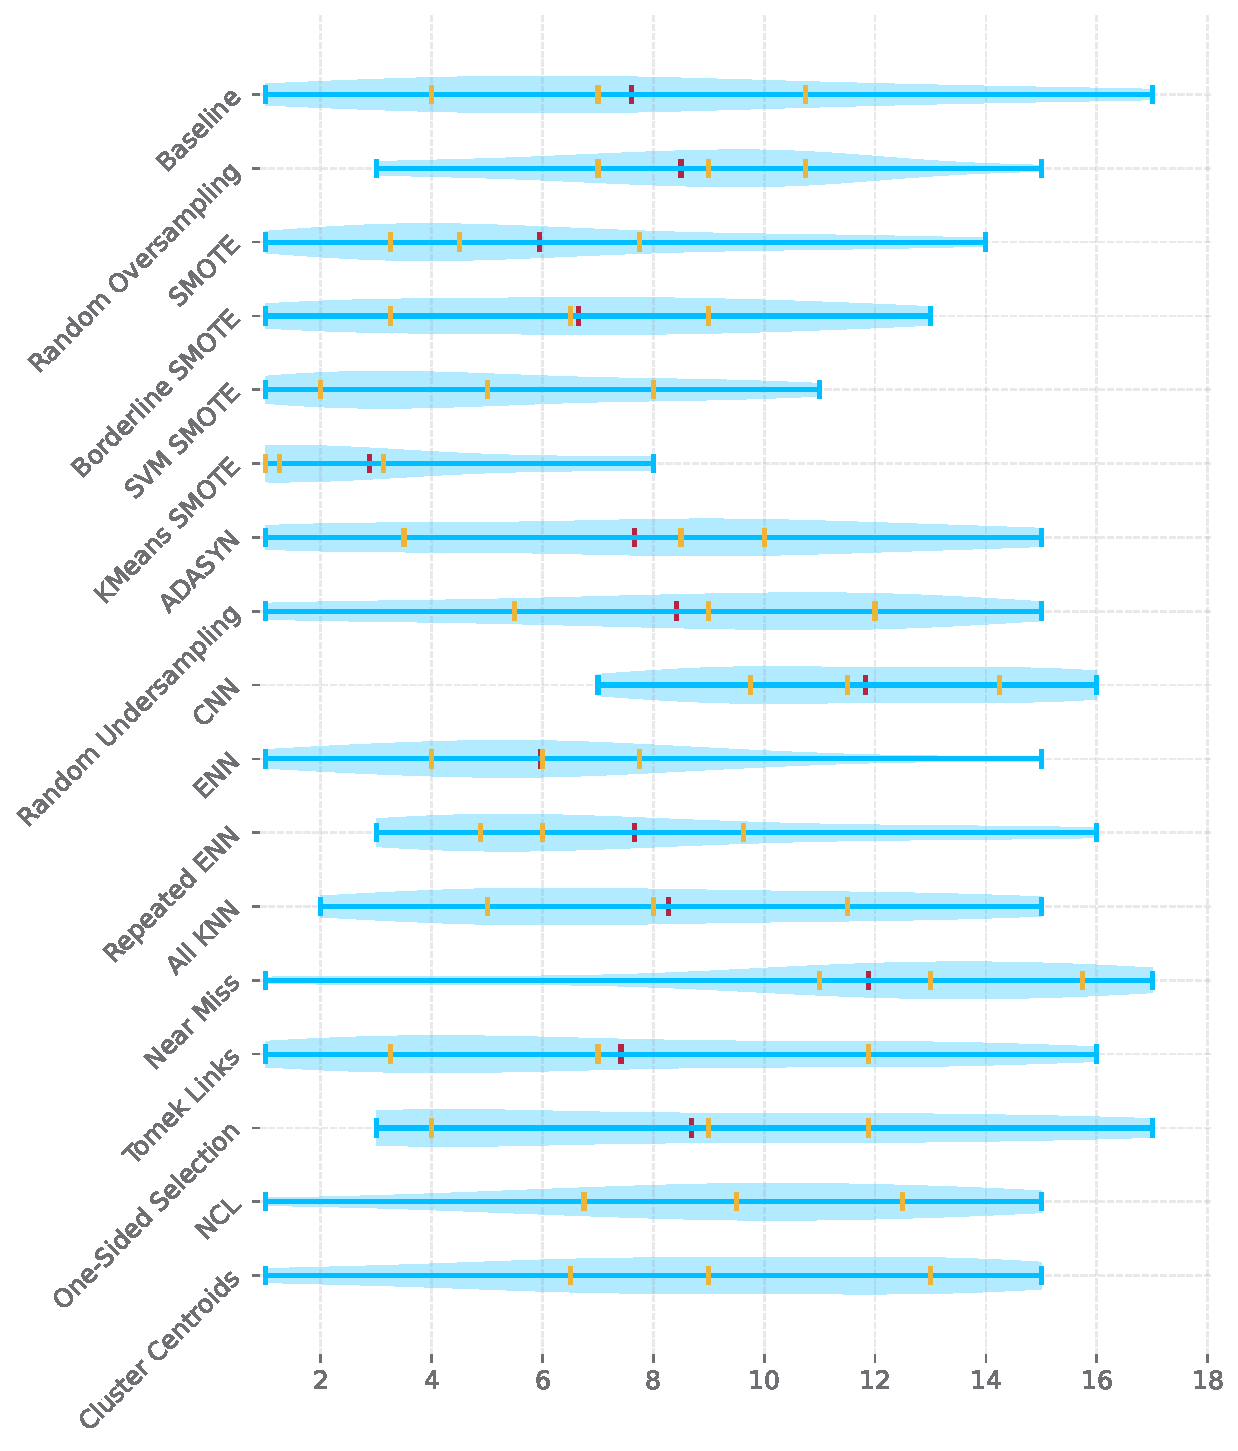
\includegraphics[width=\linewidth]{figures/roc_auc_ranks_distribution.pdf}
    \caption{
        \textbf{Distribution of Ranks for ROC AUC Evaluation Metric.} The figure shows the
        distribution of ranks computed across all datasets in the experiments. Ranks were computed
        from ROC AUC scores for each preprocessing method separately. The red mark denotes each
        method’s mean rank, and three yellow marks indicate the 25th, 50th and 75th percentile.
    }
    \label{figure:roc_auc_rank_distributions}
\end{figure}
